% example with several commonly used tex constructs
\section{Concept}
% define a marker to be referenced from outside:
\hyperdef{dabc}{concept}{[Marker:dabc.concept]}\\
As mentioned in the introduction, there are several scenarios or
use cases for the \DDA~ reflecting differing requirements and
delivery dates.
\subsection{\DDA~ use cases}
\index{Demonstrator!use cases}
\subsubsection{Detector test bed}
Detector tests with a free running system are needed to verify
that the data rates are not very much bigger than expected (dark
noise).
\subsubsection{Switched event building}
Independent of the data sources (\ABB~ or GigabitEthernet) several mechanisms for the switched
event building must be implemented and tested.
\subsubsection{DAQ framework and control systems}
There are still several options for the choice of the control system. The \xdaq~ framework
provides several communication mechanisms. The control system not necessarily must be \xdaq~ but
could be e.g. EPICS based. In such a case gateways must be implemented.
\subsubsection{\mbs~ replacement}
\index{Demonstrator!MBS} Very probably there will be no complete
replacement of the \mbs~ possible for the next years. A very big
amount of existing hardware of running \mbs~ systems cannot be
replaced neither they can be attached directly to the new DAQ
framework. At least the effort to replace the software running on
the front-end CPUs (RIO, Lynx, \mbs~) would be too big, if
possible. Instead one could envision that the \mbs~ front-end
nodes, i.e. the readout nodes, send their sub-event data peer to
peer to new event builder nodes (new \mbs~ mode). Each of these
nodes functions as sub-event receiver (Ethernet, TCP) and sends
the data for event building through the data transport network
like InfiniBand to the others and functions also as event
processor. The Ethernet input channel replaces the \ABB~input
channel.
\subsubsection{Hybrid setup}
If the system should run in production, very probably a hybrid of
\mbs~ for ancillary components and new front ends will be needed.
When running in triggered mode, the trigger of the new components
must be synchronized with the \mbs~ trigger system. In triggerless
mode the \mbs~ data must be time stamped or \mbs~ triggers must be
injected and recorded in one of the time stamped data streams by
connecting the trigger bus directly to an \FEB.
\subsubsection{Front end test bed}
The new components \FEB, \DCB, and \ABB~and their connections must be tested.
The timing system and the triggered/non-triggered mode must be tested.

\subsection{The name}
Because the systems described might be also used by other
experiments it might evolve to more than a dabcnstrator. At the
other hand it will not provide components of the front-end side
but rather provide the hooks and plug-ins to attach a big variety
of front-end systems and components. There is one principal
restriction, however, in the current design. There is nothing like
a 2nd level trigger. That means, that we assume that the full data
rate can be switched through a network for event building.
However, a congestion prevention must be provided generating dead
time for the detector readout. From this point on we have only
event filters. The front-ends might however be triggered or free
running.

The dabcnstrator as a production system would be rather a backbone. Therefore we propose a name like\\
Data Acquisition Backbone Framework {\bf DBF} (DataBaseFormat!) or {\bf ABF}\\
Data Acquisition Backbone System {\bf DBS} (Deutscher Bildungs-Server) or {\bf ABS}\\
Data Acquisition Backbone Core {\bf DABC} or {\bf ABC}\\
FAIR Acquisition Backbone {\bf FAB}

\section{\dabc~ architecture}
\begin{figure}[htb]
\centering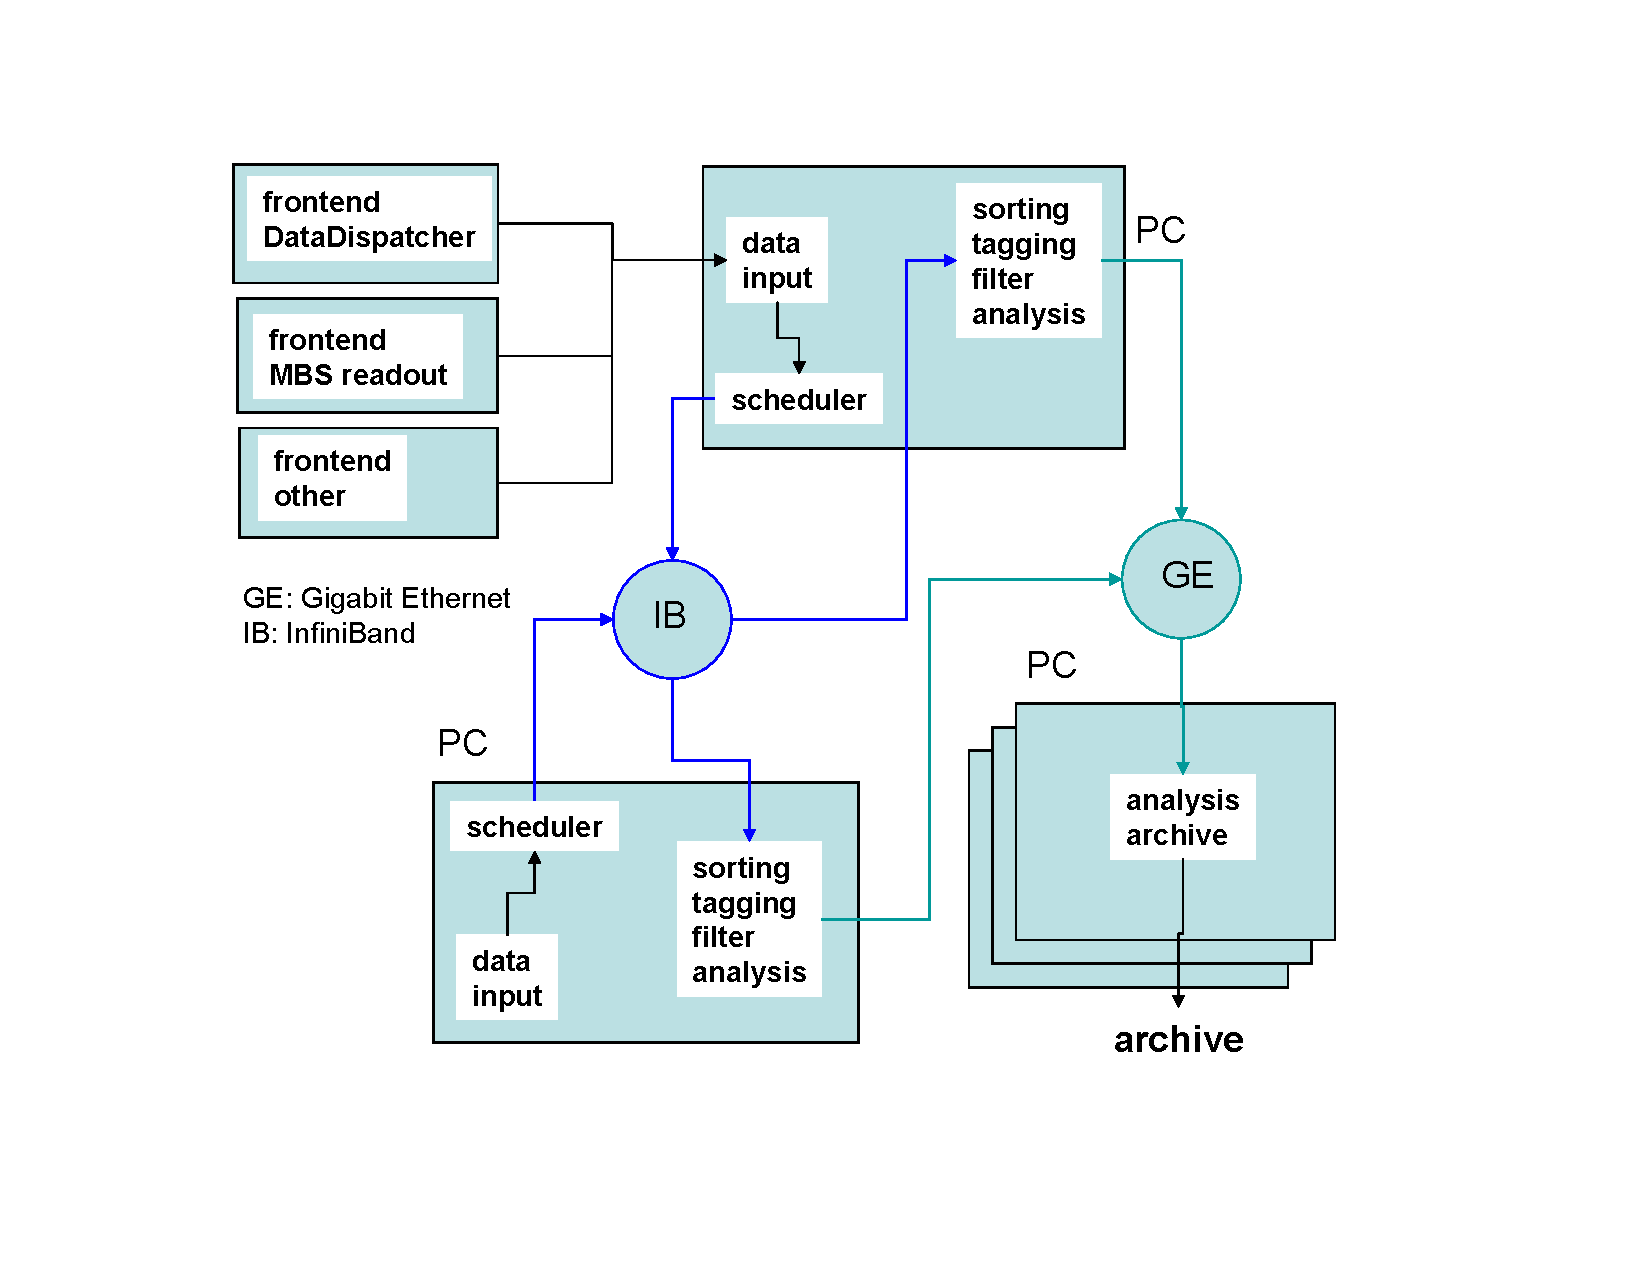
\includegraphics[width=.8\textwidth] {dabc_sw-over_4}
\caption{\dabc~ data flow and components}
\label{fig:dabc_sw-over_4}
\end{figure}

\section{Implementation phases}
One can identify four implementation phases, i.e. time scales:
\begin{compactenum}
\item \mbs~ front end support
\item Hardware tests and basic functionality of framework
\item Detector test
\item Production system
\end{compactenum}
Phase 0 might be in the beginning necessary for elementary test of the boards and the data links.
The software of phase 0 will be "experimental" and not part of the system.
\section{Requirements}
\subsection{Frontend test bed}
Phase 0, 1
\begin{figure}[htb]
\centering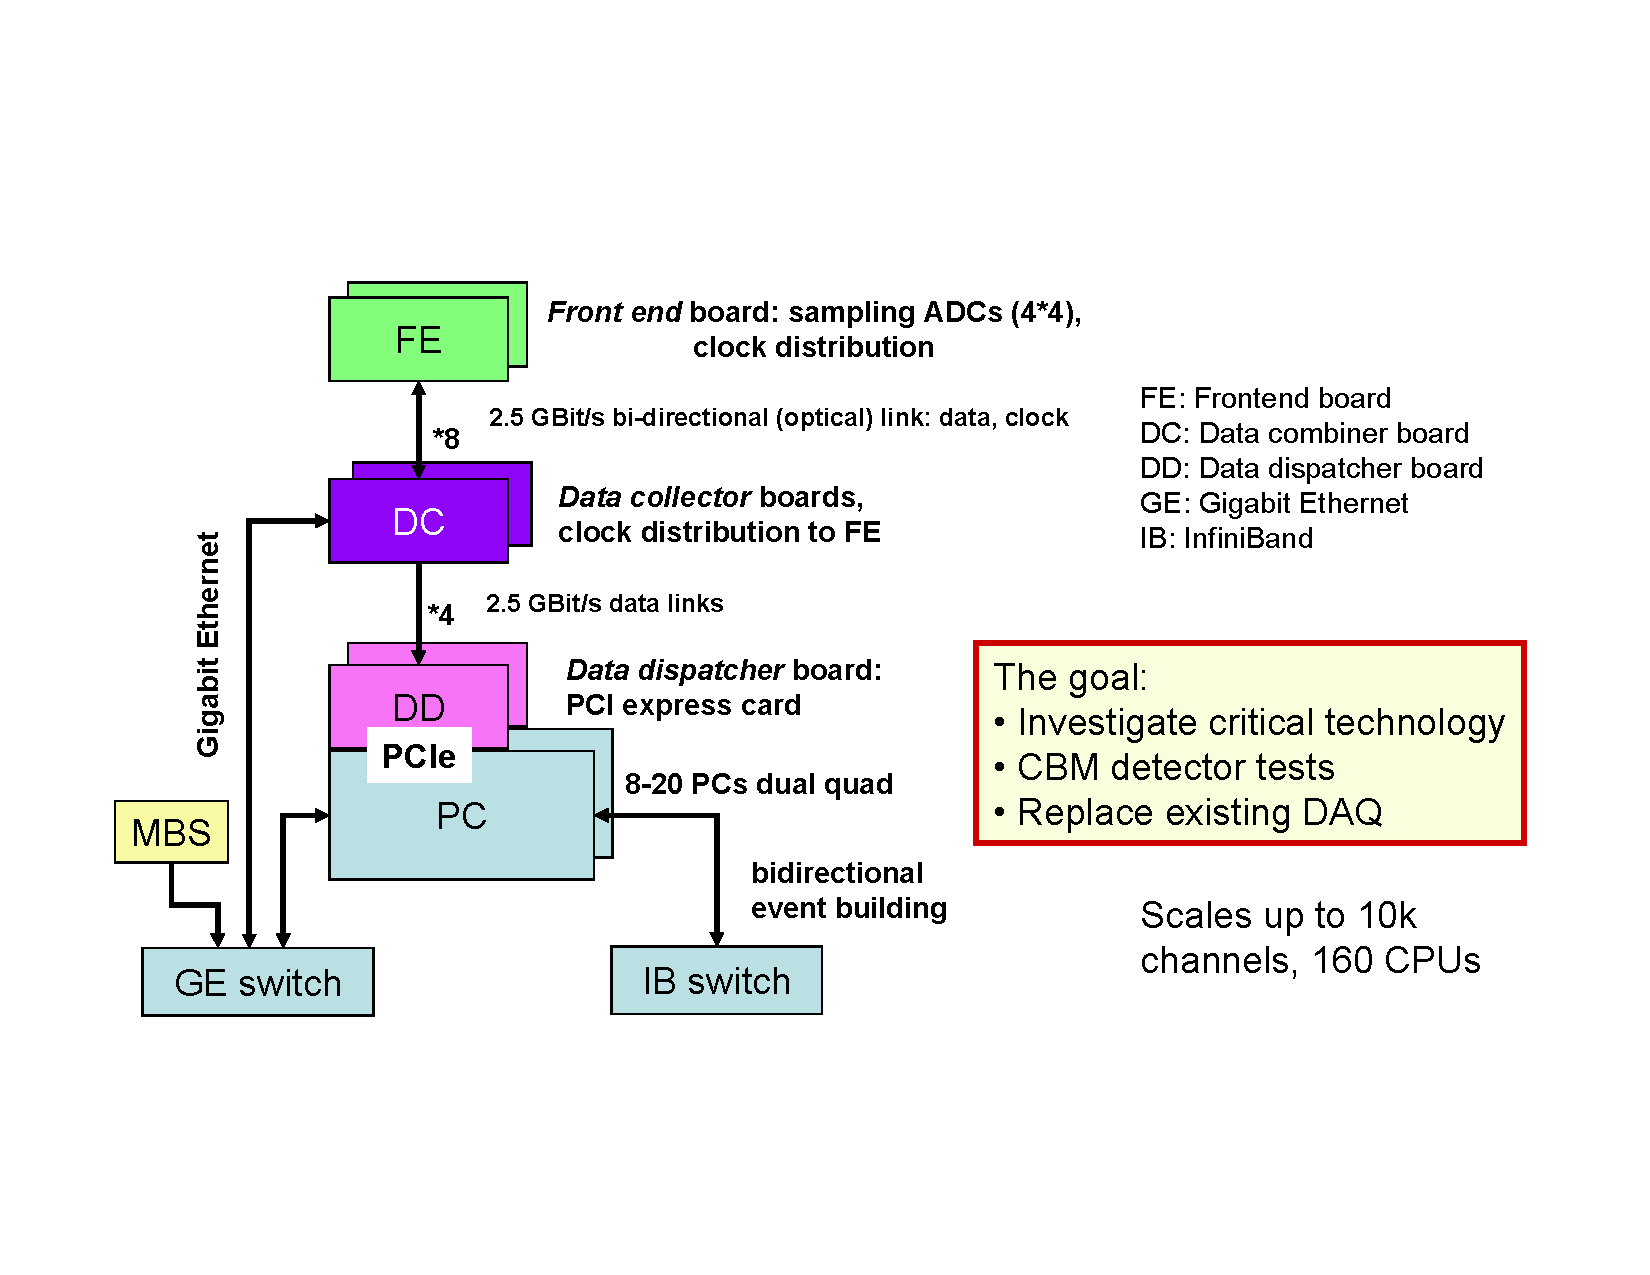
\includegraphics[width=.8\textwidth] {dabcf-all}
\caption{\dabc~ overall data processing architecture}
\label{fig:dabc-daq-over}
\end{figure}

\begin{figure}[htb]
\centering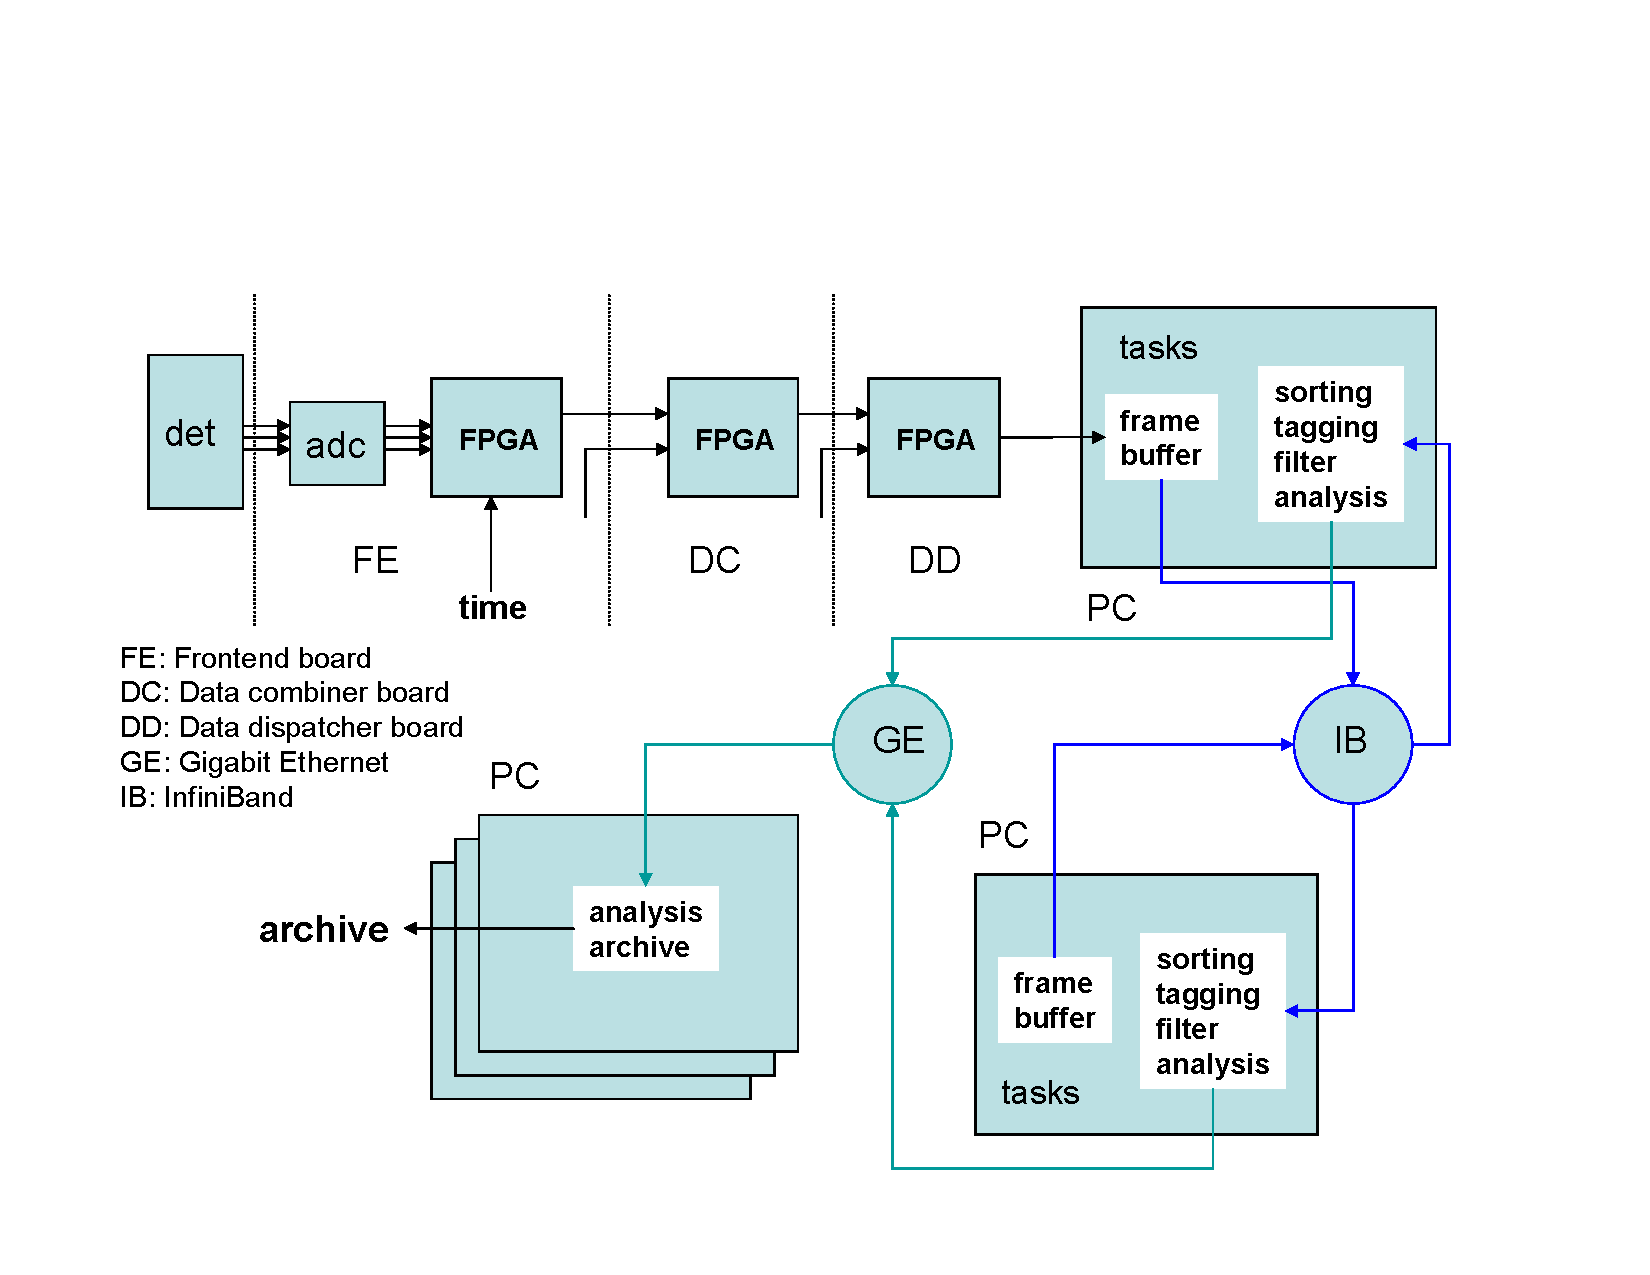
\includegraphics[width=.8\textwidth]{sw-over} % pdf file
\caption{Overall data streams architecture}
\label{fig:dabc-struct-over} % give it a name for references
\end{figure}

Fig.~\ref{fig:dabc-daq-over} shows the hardware components,
fig.~\ref{fig:dabc-struct-over} shows the data streams.
\subsection{Detector test bed}
Phase 2
\subsection{Switched event building}
Phase 2
\subsection{DAQ framework and control systems}
Phase 2
\subsection{\mbs~ front-end support}
Phase 1
\subsection{Hybrid setup}
Phase 4
\section{DABC framework requirements}

S.Linev, 23.01.2007

This is short description of required functionality, possible use cases and implementation details for some basic components of DABC framework.

\subsection{Basic overview}
I propose to build our framework as data flow model, where two main types of entities are exists: data processing units (modules) and communication (transport) layer between modules. This kind of approach used in SystemC and many ideas from this framework can be used.

\subsubsection{Transport layer}
This is major component of complete framework. Its main aim is the transport of basic data types (integer, floats) and arbitrary data packets between different parts of the distributed system. Transport can be local (inside one application) or global. Transport can be pear-to-pear or network-kind, when in addition destination address is specified. 
Interface from program code to transport should be done via 'port' entity, which should not depend from specific transport implementation. In normal operations mode user uses only port functionality to send/receive data. 
Ports are connected with each other during initialization phase. At this phase configured implementation of transport should be created and assigned for this port. 
By default, all ports are bidirectional, but one should be able to restrict port only for input or only for output. Each port can have name and, if required, data type identifier (string or number id). 
Transport layer approach gives flexibility to exchange different transports without exchange of data processing code.
Another advantage of intermediate transport layer between modules is possibility to store flowing data into the file. Later this data can be used for debugging of parts of the complete system instead of real data one can provide data from log file(s). 

\subsubsection{Processor unit (module)}
This is place for program code. All data manipulation should happen only inside modules. Communication with other modules should only be done via ports. In module constructor required number of ports should be created and registered to the module. Module should have functionality to list all ports afterwards. 

\subsubsection{Connection configuration approach}
First of all, application should be able to browse/search full hierarchy of the modules. As a result, one will have access to all ports, parameters, control values, which are available via module interface. During application startup modules should be created and local (application-wide) interconnection should be established. Connection with external nodes (or other application from the same node) can be configured locally or via control interface from operator node. 
This is static connection approach, while connections should be established before module can start working. But such approach may fail when network has dynamic nature, i.e. number of nodes or number of running processes increases/decreases during system run. Then system should be able dynamically establish new connection or brake existing ones. One possible solution is dynamic connection management, where modules could requests necessary connection to external module. For such functionality complete hierarchy of nodes/applications/processes/modules should have unique identifiers. One should avoid situations that module itself decides which transport used for connection. Connection manager should itself create appropriate transport and establish connections. 

\subsubsection{Buffer management}
As long as generic transport should support zero-copy data transfer, one should have application-wide buffer management, which takes care about buffers allocation/holding/release action. 

\subsection{Use cases}
1. Generic DAQ with several modules, connected via transport layer. One can imagine situation, when all modules run on single node, but one may also require to reconfigure same DAQ to run on several nodes. \\
2. Specific B-Net implementation. In this case one cannot use standard interface. Most probably, one should directly access transport from module to explore all functionality of specific network (for instance, MPI or verbs).

\subsection{Implementation details}
Communication port 
Here one supposes to have one common class (TTransport), which deliver interface, used by TPort class to send/receive data. TPort should not have any transport-specific code. 
Important question is usage of templates. SystemC port class is defined as template, where transferred data type is template parameter. This allows arbitrary port kinds, but complicates implementation for us, especially when one needs to communicate with different nodes and OS. I propose to support only following types: arbitrary binary buffer, integer (int64t), 64-bit double, null-terminated string. As result, one should implement four TPort::Send() methods, each for mentioned data types. In port constructor user should clearly specify which type will be used. 
Type identifier can be integer or string. Some types, deriver from binary buffer, can has it own types identifier. For instance, output port of event builder, can be identified as 'DABCFullEvent'. Probably, one can use here name, derived from data-format plugin, for instance 'MBS10\_1Event'. 
While port will have type identifier parameter, one can provide type-safety check during modules connection. Generally, types of connected port should match with each other. One also can detect error situations like two output ports are connected or similar.
Each port should have configurable size input and output queues. In the queue one store send/received values. For binary data buffer identifier is saved. 
Very important question: how we notify module when data is arrived (send). First, one should be able to use polling approach. For that appropriate flag should be defined in TPort class. One should be able to use queue size for this purpose. Second, kind of TPort::Wait() method should be implemented. It suspends receiver thread until new data is arrived. When it happens, data should be placed in receiving queue as well. Third, one can support call-back function, which is called when new data is arrived. In call-back function, defined in module class, one can immediately process incoming data. 
Seems to be, call-back approach cannot be combined with first two (wait or pool) for single port, therefore one should clearly specify port notification type at the time when port is created. One should also investigate, if notification required for the output port. 

\subsection{Transport}
Specific kind of transports (dapl, socket, pipe) should be implemented, as TTransport subclasses. Interface of TTransport class should be suited both for pear-to-pear and network-kind transport. For instance, TTransport::Send() method can have two arguments, where first is data to transfer (buffer reference or integer or float or string) and second argument is destination address (by default, -1 and ignored by peer-to-peer transport). \\
For the local (inside application) communication one need implementation which is able to transfer data between two threads. Actually, it can be single object which is associated with both input and output ports. Only buffer reference (buffer id) will be moved. Buffer itself will remain busy until receiver releases it. Actually, one can imagine situation, when several modules running in single thread and should communicate with each other. In this case call-back function approach can be most optimal (no need for additional communication threads at all).
For the global (inter-node or inter-application) communications one need of course separate objects on receiver and sender sizes. In that case transport object is responsible for release/lock of the buffers. 

\subsection{Module}
Module is aggregation of input/output ports and methods to transform data from inputs to outputs. Module should keep (be able to reproduce) list of all available ports.
Combination of several modules can be combined in one valid super-module. From outside it should be seen as normal module with several ports, inherited from sub-modules.
Probably, module should have separate list of parameters, which can be changed/viewed from outside by controlling system. 

\subsection{Buffers management}
It should be application-wide manager for buffers, allocated for data transport or just for application use. 
Because of this reason one can add some methods to TPort class, which allocates required number and size of buffers, which are suitable for transport, used for port connection. 
Buffers in manager should be grouped in subsets. Inside subset all buffers can (have to?) have same size. Buffer id (64 bit) can be combined from subset-id (16 bit) and buffer number (48 bit). 
Subset approach allows us to create one object per subset (like TBuffersSubset), not one object per buffer. This is very useful in the case, when many small buffers should be allocated. This also can be used in dapl/verbs transport implementation. There one should only register complete subset memory region and not separate memory buffers.
Actually, TBuffersSubset also can consist of set of normal buffers, where one object correspond to one buffer. 
For each buffer in subset one should keep additional information. It should be at least boolean flag, which indicate if buffer in use. One can also allow additional buffer information like data format type, individual buffer size, buffer shift and so on for each separate buffer in subset.

\subsection{Generic question} 
Which OS should be supported? Only Linux or any Unix-like? LynxOS support? 
Windows support: CYGWIN or native Win32/Win64 API or not supported at all? Probably, one can support some basic module functionality plus threading plus socket connection to enable some end-user activity on Windows. An be recognized, as low-priority task.
Do we using only glibc and pthread, or some additional library? Other thread implementations?
How we use templates? Most concern can be about list of objects like list of ports, list of parameters and so on. If we do not use template, ROOT-like approach with TNamed and TList classes should be use. This is not type-safe, but simplify search by name or similar functionality. In case of templates search methods should be implemented each time.
Do we use some basic class like TObject at all? Probably, yes. It can be useful not only in lists, but also to introduce hierarchy via parent-child relationship between objects. This provide us unique naming scheme for all objects in the system. Another solution for hierarchy: object manager, where any object property (name, config parameters and so on) stored independent from object itself.

\subsection{Requirements}
Lets summarize requirements for different components of the framework.
\subsubsection{Port}
\begin{compactitem}[$\bullet$]
\item communication entity for sending/receiving data from/to user code;
\item single TPort class, independent from specific transport implementation;
\item bi-directional or only input or only output (configurable on creation time)
\item supported data format: binary buffer, null-terminated string, integer, floats (configurable on creation time);
\item safety checks during connection: type safety, in/out comparison;
\item notification via wait/poll mechanism or via call-back (configurable on creation time);
\end{compactitem}
\subsubsection{Transport}
\begin{compactitem}[$\bullet$]
\item bidirectional data transfer between modules ports;
\item same basic TTransport class for all implementation;
\item both peer-to-peer and network in one interface;
\item local transport between modules in two threads;
\item local transport between modules in single thread;
\item global transport via pipe, socket, dapl, mpi, verbs, XDAQ peer-to-peer;
\item logging of data flow. 
\end{compactitem}
\subsubsection{Module}
\begin{compactitem}[$\bullet$]
\item keep list of ports;
\item keep list of parameters;
\item can be triggered by timer;
\item debugging possibility with use of log data;
\item unique identifier (name) over all system.
\end{compactitem}
\subsubsection{Buffer management}
\begin{compactitem}[$\bullet$]
\item buffer managed by subsets of the same size and kind of buffers;
\item TBufferSubset can has special implementation for specific transports (like verbs, dapl);
\item TPort should has methods to allocate appropriate subsets in manager;
\end{compactitem}
\subsubsection{Generic}
\begin{compactitem}[$\bullet$]
\item use of exception for error handling;
\item full support of Linux, LynxOS;
\item partial support of Windows;
\item no templates in basic transport functionality;
\item objects hierarchy via object manager or parent-child relationship;
\item basic TObject class, TList, TObjArray classes.
\end{compactitem}

